\documentclass[a4paper,ngerman]{atseminar}

\usepackage{microtype}
\usepackage{graphicx}
\usepackage{algorithm2e}
\usepackage[left]{lineno}
\usepackage{complexity}
\usepackage{csquotes}
\linenumbers

\newcommand{\N}{\ensuremath{\mathbb{N}}\xspace}
\newcommand{\BigO}[1]{\ensuremath{\operatorname{\mathcal{O}}\bigl(#1\bigr)}\xspace}
\newcommand{\BigOStar}[1]{\ensuremath{\operatorname{\mathcal{O*}}\bigl(#1\bigr)}\xspace}
\renewcommand{\deg}[1]{\ensuremath{\operatorname{\triangle}\bigl(#1\bigr)}\xspace}

\newtheorem{observation}[theorem]{\textbf{Beobachtung}}
\newtheorem{reductionrule}[theorem]{\textbf{Reduktionsregel}}

%% Please do not include packages that change the layout/size of the
%% of the document. They will be removed.

\bibliographystyle{plain}%the recommended bibstyle

% Preamble with header information 
\subject{Ausarbeitungen für das Proseminar}
\title{Algorithmen für NP-schwere Probleme}
\titlerunning{Proseminar Algorithmen für NP-schwere Probleme}%optional





%Organizer macros:%%%%%%%%%%%%%%%%%%%%%%%%%%%%%%%%%%%%%%%%%%%%%%%%%%%%%


%% do not use this field, but \summaryauthor
\author{}

%%%%%%%%%%%%%%%%%%%%%%%%%%%%%%%%%%%%%%%%%%%%%%%%%%%%%%%%%%%%%%%%%%%%%%%%%%%%%%%
%%%%%%%%%%%%%%%%%%%%%%%% begin of document %%%%%%%%%%%%%%%%%%%%%%%%%%%%%%%%%%%%
%%%%%%%%%%%%%%%%%%%%%%%%%%%%%%%%%%%%%%%%%%%%%%%%%%%%%%%%%%%%%%%%%%%%%%%%%%%%%%%
\begin{document}

\maketitle

\GERMAN

%%%%% YOUR REPORT BEGINS HERE
\section{Parametrisierte Algorithmen II}
\summaryauthor[Oliver Enes]{Oliver Enes}

\begin{abstract}
Eine kurze Zusammenfassung der Ausarbeitung. 
\end{abstract}

Hier steht der Inhalt der Ausarbeitung.

\subsection{Einleitung}

Parametrisierte Algorithmen setzen dort an, wo die klassische Komplexitätstheorie aufhört: Ziel ist es, die Laufzeit \NP-schwerer Probleme
genauer zu untersuchen.
Dazu wird die Laufzeit eines Algorithmus nicht nur in der Eingabegröße, sondern zusätzlich in einem sog. \textbf{Parameter} betrachtet.
Der Parameter ist eine Kenngröße der Probleminstanz (z.B. chromatische Zahl bei Graphen) und formalisiert die Schwere einer Probleminstanz.

\noindent
Das Konzept des Parameters motiviert die Erweiterung des Problembegriffs zum sog. \textbf{Parametrisierten Problem}:

\begin{definition}[Parametrisiertes Problem.]
  Sei $\Sigma$ ein endliches Alphabet.

  \noindent
  Ein \textbf{Parametrisiertes Problem} ist eine Sprache $L \subseteq \Sigma^* \times \N$.
  \noindent
  Die zweite Komponente einer Probleminstanz $I \in L$ wird als \textbf{Parameter} bezeichnet.
\end{definition}

\noindent
Ein Problem wird durch das Festlegen eines Parameters zum parametrisierten Problem:

\begin{table}[h]
  \centering
  \caption{Beispiele für parametrisierte Probleme}
  \begin{tabular}{ll}
    \hline
    \textbf{Problem} & \textbf{Parameter} \\
    \hline
    \textsc{Vertex Cover} & Größe des Vertex Cover \\
    \hline
    \textsc{Subset Sum} & Summe aller Elemente \\
    \hline
    \textsc{3Color} & größte Cliquengröße \\
    \hline
    \textsc{Vertex Cover} &  Minimaler Knotengrad \\
    \hline
    
  \end{tabular}
  \label{XY:tab:interessant}
  % where X is the first letter of your first name and Y is the
  % first letter of your last name.
  \end{table}

\noindent
Es sei darauf hingewiesen, dass die Parameterwahl nicht eindeutig ist. Oft wird die Lösungsgröße gewählt.

\noindent
Während der Begriff des parametrisierten Problems unabhängig von der \NP-schwere eines Problems ist, kommt diesem eine besondere
Bedeutung im Zusammenhang mit der Laufzeitanalyse \NP-schwerer Probleme zu: Laufzeiten lassen sich nun nicht nur in der Eingabegröße, sondern zusätzlich
im Parameter analysieren.
Dies begründet neue Komplexitätsklassen. Dabei ist eine für uns von zentralem Interesse:

\begin{definition}{Problemklasse \FPT.}
  Ein parametrisiertes Entscheidungsproblem heißt FPT (Fixed-Parameter-Tractable), wenn ein Algorithmus existiert,
  der alle Probleminstanzen $(x, k)$ in Laufzeit \BigO{f(k) \cdot |x|^c} löst.
  Dabei ist $c \in \N$ und $f: \N \rightarrow \N$ eine beliebige berechenbare Funktion.
\end{definition}

\begin{example}{FPT-Laufzeiten.}
  \begin{itemize}
    \item \BigO{2^k \cdot (|x|^3+42|x|)}
    \item \BigO{(43k^2+k) \cdot {|x|^2}}
    \item \BigO{|x|^{123}+12}
    \item \BigO{\varphi(k, k - 5, k - \sqrt{k}) \cdot \log(|x| + 1)} wobei $\varphi$ die Ackermann-Funktion ist.
  \end{itemize}
\end{example}

\noindent
Die Laufzeit ist also insbesondere polynomiell in der Instanzgröße und nahezu beliebig im Parameter.
Lässt sich also für ein parametrisiertes Entscheidungsproblem ein \FPT-Algorithmus finden, so kann dieser höchstens im Parameter superpolynomiell sein.
Dabei wird eine wünschenswerte Eigenschaft des Parameters deutlich: der Parameter formalisiert die \enquote{Gutartigkeit} eines Problems, indem er den potentiellen superpolynomiellen
Anteil der Laufzeit eines Algorithmus durch sich beschränkt. Dabei sei angemerkt, dass die Parameterwahl zentral für diese Eigenschaft ist.
So kann für das gleiche "klassische" Problem als parametrisiertes Problem in einem Parameter ein \FPT-Algorithmus existieren, während für eine andere Wahl
des Parameters kein solcher Algorithmus bekannt ist.

Oft interessiert man sich nur für den Anteil der Laufzeit, der vom Parameter abhängt. In diesem Fall lässt sich vereinfacht
$\BigOStar{f(k)}$ schreiben, um eine \FPT-Laufzeit zu formulieren, dessen polynomieller Anteil beliebig ist.
Es ist also $\BigOStar{f(k)} = \bigcup_{c \in \N} \BigO{f(k) * |x|^c}$.

\subsection{Problemkerne und Problemkernreduktion}

Eine wichtige Technik im Bereich der parametrisierten Algorithmen ist die Bildung sog. Problemkerne.
Ein Problemkern entsteht, indem eine gegebene Instanz eines parametrisierten Problems derart reduziert wird, dass der triviale/in polynomieller Zeit lösbare
Teil der Instanz entfernt wird, sodass die so entstehende Instanz nur noch den Teil enthält, dessen Lösung superpolynomielle Zeit beansprucht.
\noindent
Dabei fordern wird jedoch, dass die Größe des Problemkerns nur vom Parameter abhängt.

\noindent
Formal ergibt sich die

\begin{definition}{Problemkerne und Problemkernreduktion.}
  Sei $L  \subseteq \Sigma^* \times \N$ ein parametrisiertes Problem.
  Eine Problemkernreduktion $ \Phi: \Sigma^* \times \N \rightarrow \Sigma^* \times \N $ ist eine Funktion, sodass:
  \begin{itemize}
      \item $I \in L \iff I' := \Phi(I) \in L $ (\textbf{Äquivalenz}).
      \item $|I'| \leq f(k)$ für eine beliebige Funktion $f: \N \rightarrow \N$ (\textbf{Beschränktheit}).
      \item $\Phi$ ist polynomiell in $|x| + k$ berechenbar (\textbf{Berechenbarkeit}).
  \end{itemize}
\end{definition}

\noindent
Der Leser sei darauf hingewiesen, dass $\Phi$ nicht nur in $|x|$ sondern auch in $k$ polynomiell berechenbar sein muss.
Dies lässt sich einsehen durch die
\begin{observation}

  Eine parametrisierte \textsc{Vertex Cover} Instanz, wobei die Lösungsgröße der Parameter ist, lässt sich mittels eines
  Bruteforce Algorithmus $\mathcal{A}$ in $\BigO{\binom{n}{k}} \preceq \BigO{n^k}$ lösen.

  \noindent
  Entsprechend lässt sich eine Reduktion $\tilde{\Phi}$ konstruieren, die Instanzen mittels $\mathcal{A}$ löst und dann triviale
  Problemkerne zurückgibt.
  Damit gelten dann (\textbf{Äquivalenz}) und (\textbf{Beschränktheit}), jedoch hat $\tilde{\Phi}$ exponentielle Laufzeit in $k$.
  \noindent
  Durch die Aufweichung der Laufzeit-Bedingung ist es also möglich, Reduktionen zu konstruieren, die auch "schwere" Teile einer Instanz lösen.
  Dies widerspricht der Idee eines Problemkerns, der eben die Teile einer Instanz enthält, die superpolynomielle Laufzeit verursachen.
  Unabhängig davon, birgt eine derartige Aufweichung der Laufzeit auch im praktischen Einsatz Nachteile: Wenn die Problemkernreduktion selbst
  schon exponentielle Laufzeit benötigt, besteht kein großer Sinn, zuerst einen Problemkern zu berechnen und diesen dann in superpolynomieller Zeit
  zu lösen.
\end{observation}

\noindent
Ein gängiges Vorgehen ist also, zunächst einen - möglichst kleinen - Problemkern in polynomieller Zeit zu berechnen, dessen Lösung zwar tendenziell exponentiell viel Zeit benötigt,
durch die Größe des Problemkerns aber im Vergleich zur ursprünglichen Instanz in guter Zeit gelöst werden kann.

\noindent
Wir wollen die Bildung eines Problemkerns exemplarisch am Problem \textsc{Vertex Cover} verdeutlichen. Dieses definieren wir als
parametrisiertes Entscheidungsproblem \textsc{k Vertex Cover}:

\begin{definition}{Problem \textsc{k Vertex Cover}.}
  \\
  \begin{tabular}{ll}
    \textbf{Gegeben:} & einfacher, ungerichteter Graph  $G = (V, E), \quad k \in \N$. \\
    \textbf{Parameter:} & Lösungsgröße k. \\
    \textbf{Gesucht:} & $M \subseteq V$, sodass $ |M| \leq k $ und $ \forall e \in E : e \cap M \neq \emptyset$.
  \end{tabular}
\end{definition}

\begin{example}[Problemkernreduktion für k \textsc{Vertex Cover}]
    Die Problemkernreduktion besteht aus einer Reihe sog. Reduktionsregeln. Dabei handelt es sich um eine in sich geschlossene
    Vorschrift, wie eine Instanz in eine andere überführt wird.
    Wichtig ist, neben der polynomiellen Laufzeit die sog. Äquivalenzbedingung (im Englischen oft als "safeness" bezeichnet).
    Diese fordert, dass eine reduzierte Instanz genau dann eine Ja-Instanz ist, wenn die ursprüngliche Instanz eine Ja-Instanz ist.

    \noindent
    Hingegen ist die Beschränktheit der Instanzgröße durch den Parameter nicht gefordert.

    \begin{reductionrule}
      \label{OE:reduction:1}
      Ist $(G, k)$ eine k-\textsc{Vertex Cover} Instanz und $U \subseteq V(G)$, sodass $ (U \times V(G)) \cap E(G) = \emptyset $ ist, so ist $(G - U, k)$
      eine äquivalente Instanz.
    \end{reductionrule}
    \begin{proof}
      $U$ ist eine Menge an isolierten Knoten in $G$. Diese tragen nichts zur Kantenabdeckung bei.
    \end{proof}

    \begin{reductionrule}
      \label{OE:reduction:2}
      Ist $(G, k)$ eine k \textsc{Vertex Cover} Instanz mit Parameter $k$ und $v \in V(G)$ mit Grad $\deg{v} \geq k + 1$,
      so ist $(G - v, k - 1)$ eine äquivalente Instanz. $v$ ist im Vertex Cover M von $G$ enthalten.
    \end{reductionrule}
    \begin{proof}
      Dass $v$ im Vertex Cover enthalten ist, zeigen wir wie folgt:
      angenommen, $v \notin M$. Dann muss die Nachbarschaft $N(v)$ in M enthalten sein. Jedoch ist $|N(v)| = \deg{v} \geq k + 1 > k$.


      \noindent
      Die Äquivalenz der Instanzen sieht man folgendermaßen ein:

      \noindent
      Ist $(G, k)$ eine Ja-Instanz mit Vertex Cover "M" und $v \in V(G)$ mit $\deg{v} \geq k + 1$, so ist $M' := M \backslash \{v\}$ ein Vertex Cover in $G - v$.
      Insbesondere ist $|M'| = |M| - 1 \leq k -1$.
      Damit löst $M'$ die reduzierte Instanz $(G - v, k - 1)$.

      \noindent
      Sei nun $(G - v, k - 1)$ eine reduzierte Vertex Cover Instanz mit Lösung $M'$. Durch die Hinzunahme von $v$ entsteht der Graph $G$.
      Alle neu hinzugekommenden Kanten werden durch den Knoten $v$ abgedeckt.
      Damit ergibt sich als Vertex Cover für $G$ die Menge $M := M' \cup \{v\}$.
      Es ist $|M| = |M'| + |\{v\}| = |M'| + 1 \leq k$. Damit löst $M$ die Instanz $(G, k)$.
    \end{proof}

    \noindent
    Durch Anwendung von (\ref{OE:reduction:2}) können natürlich isolierte Knoten entsehen. Diese können wiederum mit Hilfe von (\ref{OE:reduction:1}) entfernt
    werden.
    Reduktionsregeln können (und sollten) also mehrmals angewandt werden. Lässt sich eine Reduktionsregel nicht mehr anwenden, selbst nachdem andere Reduktionsregeln
    die Instanz weiter reduziert haben, sagt man, dass die Reduktionsregel \textbf{erschöpfend} angewendet worden ist.

    \noindent
    Wir kommen zur letzten Reduktionsregel:

    \begin{reductionrule}
      Ist $(G, k)$ eine k \textsc{Vertex Cover} Instanz mit $\deg{v} \leq k$ für alle $ v \in V(G)$ und $|E(G)| \geq k^2$, so ist $(G, k)$
      eine Nein-Instanz. Gib eine triviale Nein-Instanz zurück. 
    \end{reductionrule}
    \begin{proof}
      Wir zeigen, dass eine Menge an $k$ Knoten nicht ausreichen kann, um alle Kanten in $G$ abzudecken.
      \noindent
      Maximale Abdeckung wird erreicht, wenn die Kantenmengen der einzelnen Knoten in $M$ disjunkt sind und der Grad aller Knoten maximal ist.
      
      \noindent
      Dann lassen sich $\sum_{v \in M}{\deg{v}} = \sum_{v \in M}{k} = k^2$ abdecken.
      \noindent
      Da aber $|E(G)| > k^2$, kann folglich kein Vertex Cover der Größe $k$ existieren.
    \end{proof}
\end{example}






\subsection{Abschnitt der Ausarbeitung}

\subsubsection{Unterabschnitt der Ausarbeitung}


\paragraph{Bitte keine Paragraphen verwenden!}


\begin{figure}[h]
 \centering
 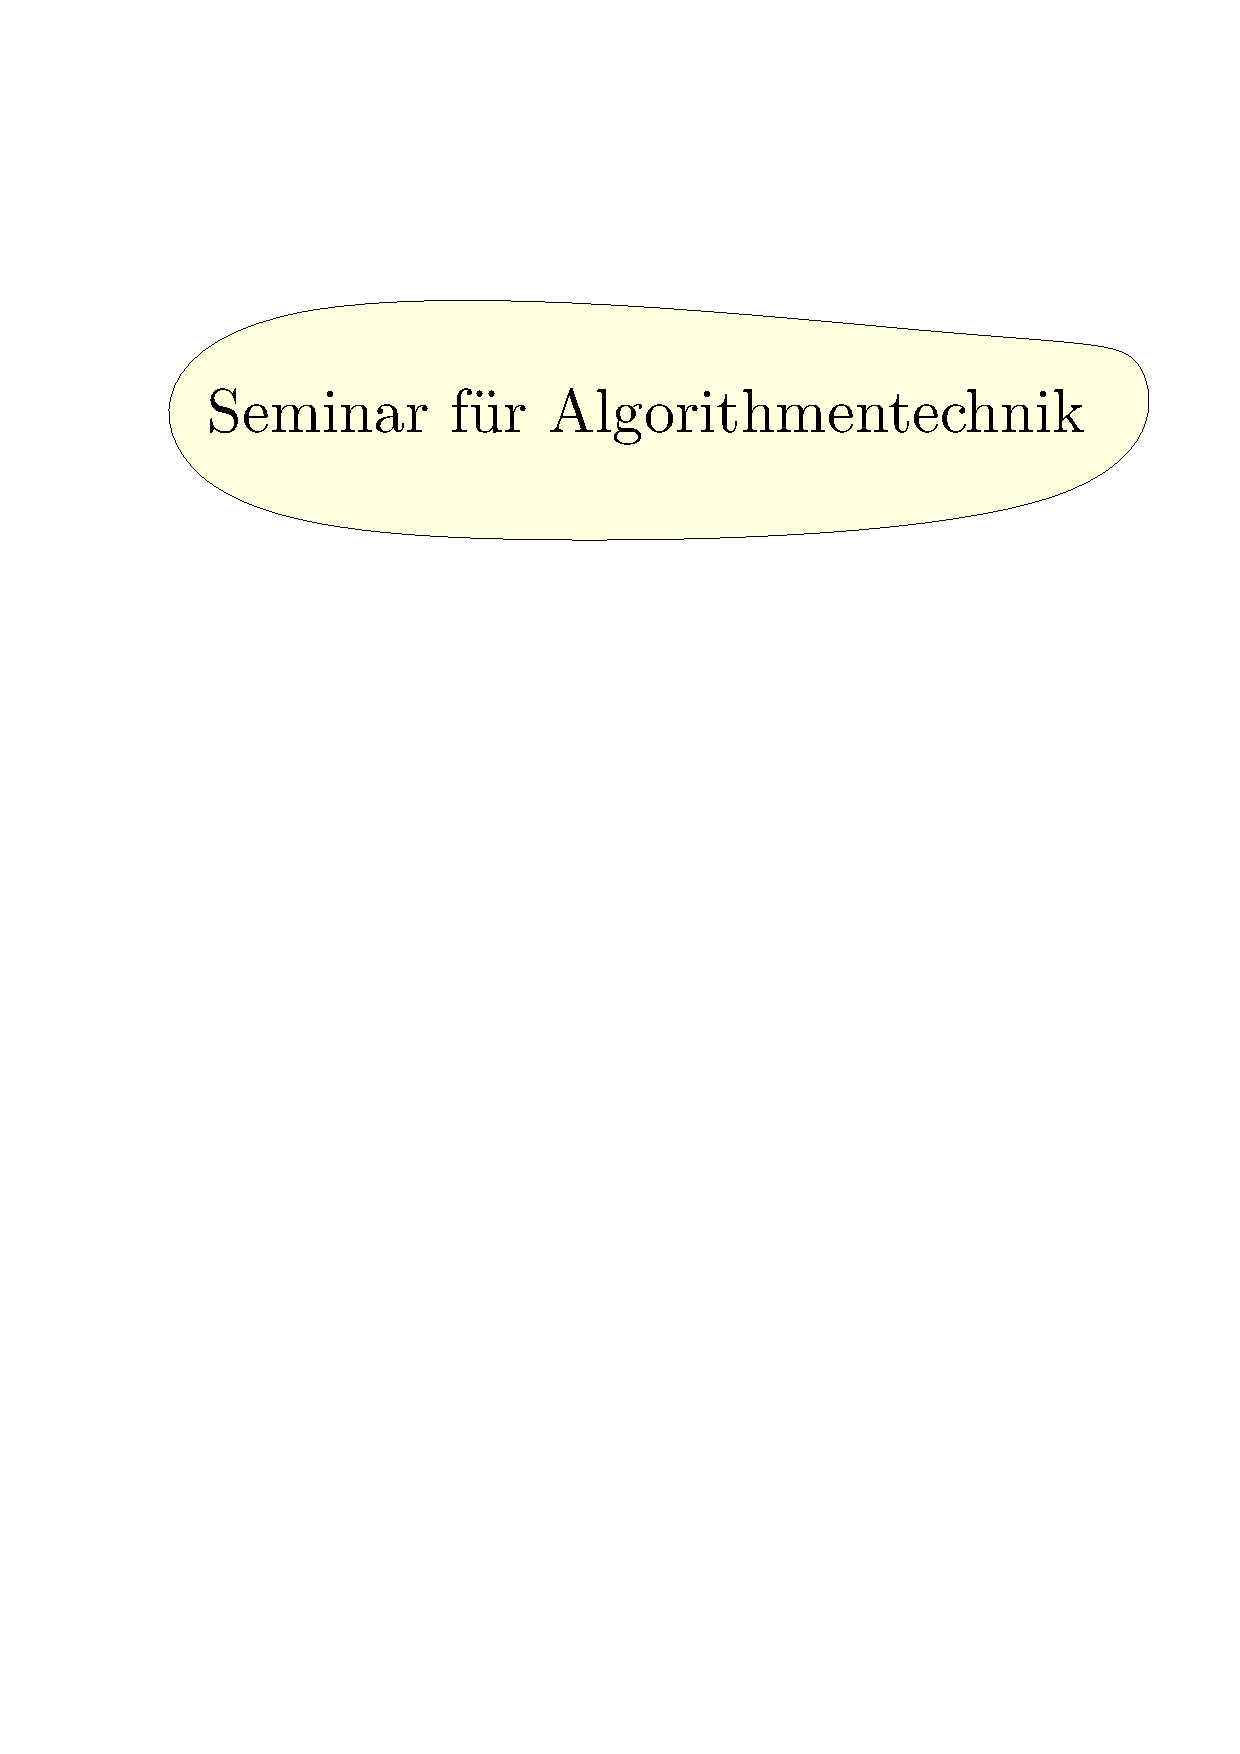
\includegraphics[scale = 0.7]{./picture}
 \caption{Dies ist die Beschreibung der Abbildung: Kurze Erklärung
was zu sehen ist.}
 \label{XY:fig:picture}
 % where X is the first letter of your first name and Y is the
% first letter of your last name.
\end{figure}

\begin{table}[h]
\centering
\caption{Tabellen haben Überschriften.}
\begin{tabular}{l|ll}
  \textbf{Zelle11} & \textbf{Zelle12} & \textbf{Zelle13} \\
  \hline
  \textbf{Zelle21} & Zelle22 & Zelle23 \\
  \textbf{Zelle31} & Zelle32 & Zelle33 \\
  
\end{tabular}
\label{XY:tab:interessant}
% where X is the first letter of your first name and Y is the
% first letter of your last name.
\end{table}



\begin{algorithm}[H]
\caption{Greedy}
\KwIn{Menge $\mathcal{C}$ aller Kreise in $G=(V,E)$.}
\KwOut{ Kreisbasis minimalen Gewichts von $G$.}
Sortiere $\mathcal{C}$ aufsteigend nach Gewicht zu $C_1,\ldots,C_k$\; 
$\mathcal{B}^\star$ $\leftarrow$ $\emptyset$\; %
  \For{$i = 1$ \KwTo $k$}{ %
    \If{$\mathcal{B}^\star \cup \{C_i\}$ linear unabhängig}{ %
      $B^\star$ $\leftarrow$ $B^\star \cup \{C_i\}$\; 
    }
} %
\end{algorithm}

\begin{theorem}[Titel des Theorems (optional)]
 Die Aussage des Theorems.
\end{theorem}

\begin{proof}
 Der Beweis für das Theorem.
\end{proof}

\begin{example}
 Dies ist ein Beispiel.
\end{example}


\begin{lemma}[Titel des Lemmas (optional)]
 Die Aussage des Lemmas
\end{lemma}

\begin{corollary}[Titel des Korollar (optional)]
 Ein Korollar.
\end{corollary}


\begin{definition}[Titel der Definition(optional)]
Inhalt der Definition
\end{definition}

Das erste Beispiel \cite{example1}, das zweite Beispiel
\cite{example2} und  das dritte Beispiel \cite{example3, example4}
für eine Referenz.

\subsection{Zweiter Abschnitt}


\begin{definition}[Titel der Definition(optional)]
Inhalt der Definition
\end{definition}





\bibliography{references}



%%%%% YOUR REPORT ENDS HERE




\end{document}
